\chapter{Thiết kế Facebook chatbot với Chatfuel}
\textit{Chatfuel} là một công cụ tạo chatbot miễn phí (cho quy mô nhỏ) giúp xây dựng nhanh một chatbot trên mạng xã hội Facebook. Chatfuel mạnh mẽ không chỉ ở giao diện trực quan, mà còn ở việc hỗ trợ JSON dành cho việc mở rộng thuật toán bằng lập trình.\par

\section{Nền tảng Chatfuel}
Để tạo chatbot với Chatfuel, trước hết cần có quyền \textit{quản trị viên} (administrator) của một trang Facebook (Facebook fanpage). Sau khi đăng nhập vào {\color{mTeal}chatfuel.com}, giao diện của Chatfuel tương tự như hình \ref{fig:fig-c3-dashboard}. Trong đó:
\begin{enumerate}[label=\textbf{(\arabic*)},align=left,left=0cm..0cm,itemindent=*]
	\item \textbf{Create from Template}: Tạo một chatbot mới từ mẫu có sẵn, hoặc một chatbot trắng.
	\item Menu xuất hiện ở các chatbot đã tạo cho phép thực hiện các thao tác cơ bản như \textit{đổi tên} (rename), \textit{sao chép} (copy), \textit{xóa} (delete).
	\item Chọn chatbot để truy cập giao diện làm việc chính của Chatfuel.
\end{enumerate}\par

\begin{figure}[htb!]\centering
	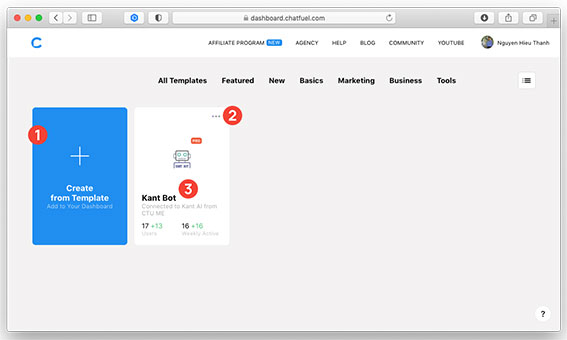
\includegraphics[width=15cm]{chatfuel/dashboard}
	\caption{Giao diện bắt đầu của Chatfuel}
	\label{fig:fig-c3-dashboard}
\end{figure}\par

\subsection{Giao diện làm việc}
Sau khi ch người dùng được chuyển tới giao diện làm việc của Chatfuel (hình \ref{fig:fig-c3-grow}), trước hết là mục \textit{Grow} – chứa các thông tin cơ bản để phát triển chatbot như \textit{trang Facebook đã kết nối} (connected page, mục \textbf{(8)}), cách bot trả lời lại một số tin nhắn người dùng thường gửi, các \textit{tiện ích mở rộng} (plugin).\par
\begin{figure}[htb!]\centering
	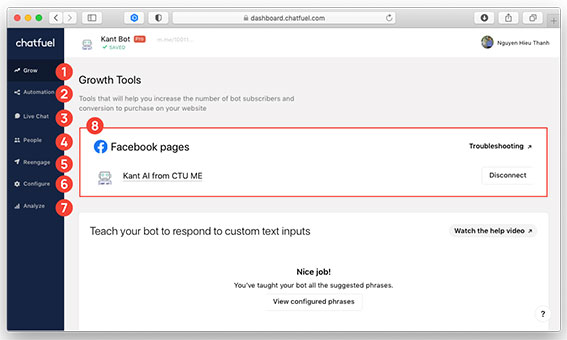
\includegraphics[width=15cm]{chatfuel/grow}
	\caption{Giao diện làm việc chính của Chatfuel}
	\label{fig:fig-c3-grow}
\end{figure}\par

Bên phải màn hình là thanh điều hướng:
\begin{enumerate}[label=\textbf{(\arabic*)},align=left,left=0cm..0cm,itemindent=*]
	\item \textbf{Grow}: Trang bắt đầu, chứa các thông tin cơ bản và công cụ giúp phát triển chatbot.
	\item \textbf{Automation}: Các thiết đặt trả lời tự động.
	\item \textbf{Live Chat}: Hiển thị các tin nhắn yêu cầu trò chuyện với quản trị viên (các vai trò trên chatbot được thiết đặt ở mục \textbf{(6)}).
	\item \textbf{People}: Hiển thị danh sách và các thuộc tính, thông tin người dùng đã tương tác với chatbot.
	\item \textbf{Re-engage}: Cho phép tương tác lại với các người dùng đã sử dụng chatbot, đã lâu không tương tác, chưa hoàn thành việc nào đó (theo điều kiện tự thiết đặt)...
	\item \textbf{Configure}: Cài đặt cho chatbot, bao gồm múi giờ của chatbot, menu hoạt động, các thành viên có thể quản lý bot...
	\item \textbf{Analyze}: Các phân tích định lượng và gợi ý cho việc phát triển bot.
\end{enumerate}

\subsubsection{Mục Automation}
Phần này cung cấp các công cụ để tạo ra những cuộc hội thoại hoàn toàn tự động và linh hoạt (hình \ref{fig:fig-c3-flows}):
\begin{enumerate}[label=\textbf{(\arabic*)},align=left,left=0cm..0cm,itemindent=*]
	\item \textbf{Flows}: Thiết đặt trả lời tự động thông qua các khối trực quan, việc này tương tự với biểu diễn thuật toán bằng biểu đồ.
	\item \textbf{Blocks}: Tạo ra các "khối" tin nhắn xác định, có thể dễ dàng \textit{điều hướng} (navigate) qua lại với Flows.
	\item \textbf{Set up AI}: Đặt các quy tắc trả lời tự động (hoặc điều hướng sang Block, Flow) thông qua việc nhận dạng các cụm từ, tin nhắn...
\end{enumerate}\par
\textbf{\textit{Flows}} cho phép sử dụng cấu trúc rẽ nhánh (nếu... thì...) và có thể điều hướng rất linh hoạt thông qua giao diện chỉnh sửa trực quan, do đó, nó thường được lựa chọn cho các cuộc hội thoại dài và phức tạp. Một flow có thể đảm nhiệm một mảng lớn của chatbot. Điển hình là các phần hướng dẫn, hỏi đáp (Q-A), khảo sát... Tuy nhiên, do vẫn còn ở giai đoạn thử nghiệm, nên flow vẫn chưa được hoàn thiện về mặt hiệu năng, đặc biệt là giao diện chỉnh sửa không ổn định khi làm việc với những flow mang tính phức tạp. Giao diện Flows gồm có hai phần: \textbf{(4)} danh sách các flow và \textbf{(5)} khu vực thiết kế flow với các nút lệnh \textbf{(6)} (hình \ref{fig:fig-c3-flows}).\par

\begin{figure}[htb!]\centering
	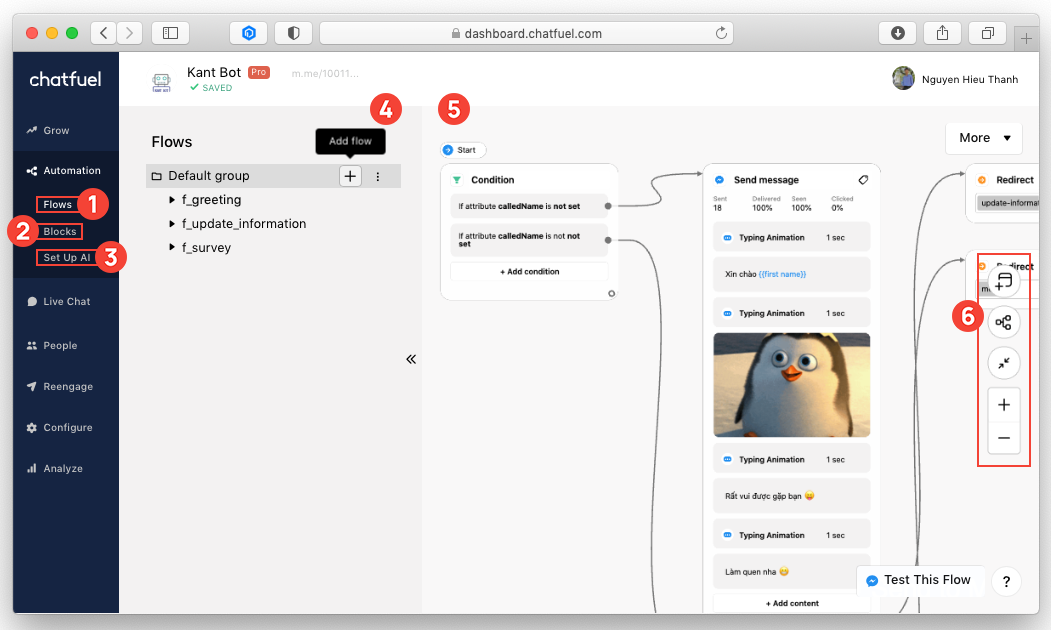
\includegraphics[width=15cm]{chatfuel/flows}
	\caption{Thiết đặt trả lời tự động với chức năng \textit{Flows}}
	\label{fig:fig-c3-flows}
\end{figure}\par

\textbf{\textit{Blocks}} cho phép trả lời tự động thông qua các khối được thiết đặt từ trước. Blocks sử dụng giao diện chỉnh sửa tuyến tính và không hỗ trợ cấu trúc rẽ nhánh như Flows, nên một block không thể đảm nhận nhiều công việc. Khi chưa có flow, block thường được dùng riêng lẻ để gọi JSON API – thành phần quyết định các cấu trúc rẽ nhánh và điều hướng. Hiện nay, block thường được sử dụng cho các giao tiếp đơn giản, gửi các hình ảnh có sẵn, gọi JSON API cho các thuật toán phức tạp... Giao diện thiết lập block tương tự hình \ref{fig:fig-c3-blocks}, trong đó: \textbf{(1)} chứ các nhóm và các block, \textbf{(2)} không gian biên tập block.\par
\begin{figure}[htb!]\centering
	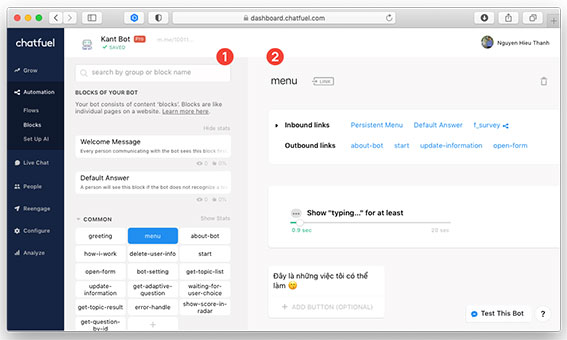
\includegraphics[width=15cm]{chatfuel/blocks}
	\caption{Thiết đặt trả lời tự động với chức năng \textit{Blocks}}
	\label{fig:fig-c3-blocks}
\end{figure}\par

Phần \textbf{\textit{Set up AI}} cho phép kết hợp các flows và blocks lại với nhau, thông qua việc nhận dạng từ ngữ nhận được, bot sẽ trả lời bằng \textit{tin nhắn văn bản} (text messages) hoặc \textit{chuyển hướng} (re-direct) sang các phần khác. Tính năng này đặc biệt hiệu quả do ta có thể dạy bot cách phản hồi thật chính xác theo mong muốn của mình. Ngoài ra, ở mục \textit{Grow}, Chatfuel sẽ gợi ý một số cụm từ, tin nhắn mà người dùng thường xuyên gửi đến, giúp bao quát hóa việc học tập của AI. Ở giao diện này (hình \ref{fig:fig-c3-set-up-ai}), người dùng có thể thêm mới một \textit{quy tắc} (rule – \textbf{(1)}), sau đó nhập các cụm từ vào mục \textbf{(2)} và thiết lập cách phản hồi của bot ở mục \textbf{(3)}.\par
\begin{figure}[htb!]\centering
	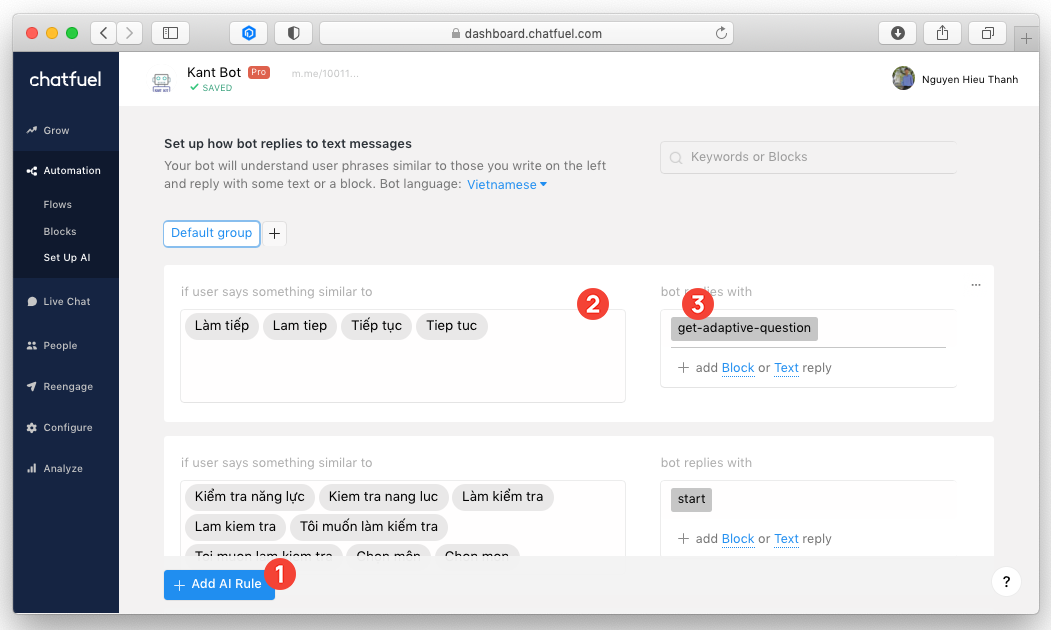
\includegraphics[width=15cm]{chatfuel/set-up-ai}
	\caption{Thiết đặt trả lời tự động với chức năng \textit{Set up AI}}
	\label{fig:fig-c3-set-up-ai}
\end{figure}\par

\subsubsection{Mục People}
Mục people (hình \ref{fig:fig-c3-people}) cung cấp danh sách chi tiết người dùng đã tương tác với bot, các thuộc tính có sẵn và các thuộc tính tự thiết lập:
\begin{enumerate}[label=\textbf{(\arabic*)},align=left,left=0cm..0cm,itemindent=*]
	\item Hiển thị danh sách người dùng và các thuộc tính, thời gian truy cập... Phần này có thể tùy chỉnh danh sách các cột tùy theo nhu cầu sử dụng.
	\item Cung cấp chức năng lọc danh sách người dùng theo nhóm: người dùng chủ động nhắn tin với chatbot, người dùng nhấn vào quảng cáo, người dùng bình luận các bài đăng của fanpage...
	\item Quản lý chung danh sách người dùng của chatbot, cụ thể: lưu vào nhóm nào đó, xóa người dùng, xuất dưới dạng tệp CSV (Comma-separated values).
\end{enumerate}\par

\begin{figure}[htb!]\centering
	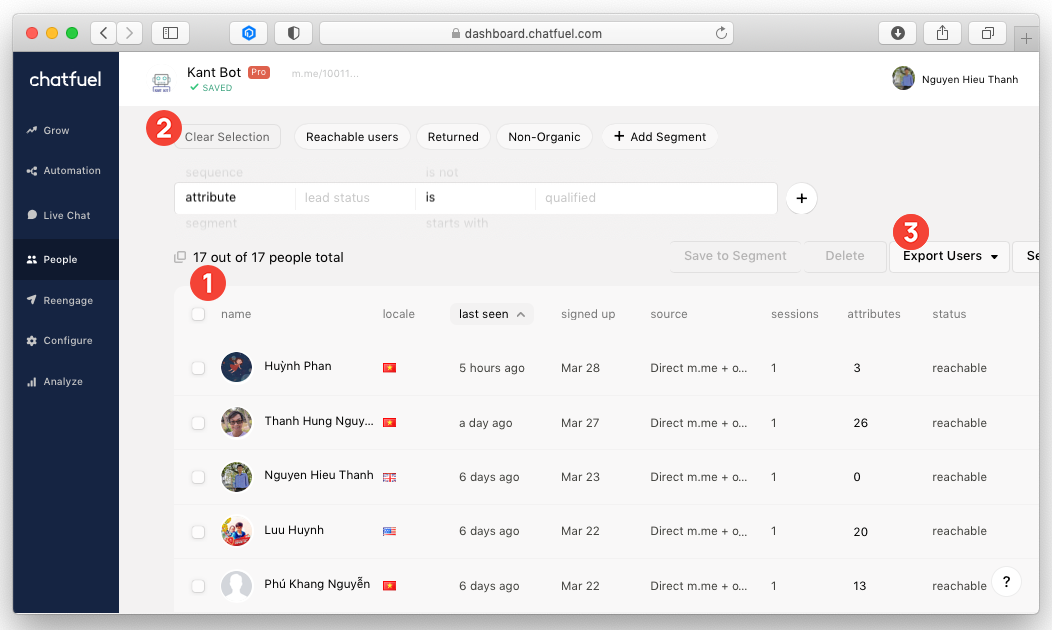
\includegraphics[width=15cm]{chatfuel/people}
	\caption{Giao diện danh sách người dùng đã tương tác với bot}
	\label{fig:fig-c3-people}
\end{figure}\par

\subsubsection{Mục Re-engage}
Chức năng này cung cấp nhiều cách để tương tác tự động với (nhóm) người dùng của chatbot thông qua việc gửi tin nhắn đến một nhóm người nhận và gợi ý người dùng đăng ký vào nhóm thông báo. Chatfuel cho phép \textbf{(1)} gửi thủ công ngay lập tức, \textbf{(2)} lên lịch cho tin nhắn, \textbf{(3)} gửi tin nhắn theo một sự kiện được thiết lập sẵn (sau 24 giờ không tương tác, khi thay đổi một thuộc tính...), \textbf{(4)} tự động gửi tin nhắn từ các nguồn bên ngoài chatfuel (qua JSON API). Tin nhắn được thiết kế và gửi từ \textit{re-engage} hoàn toàn tương tự với giao diện thiết kế \textit{blocks} \textbf{(5)}.\par

\begin{figure}[htb!]\centering
	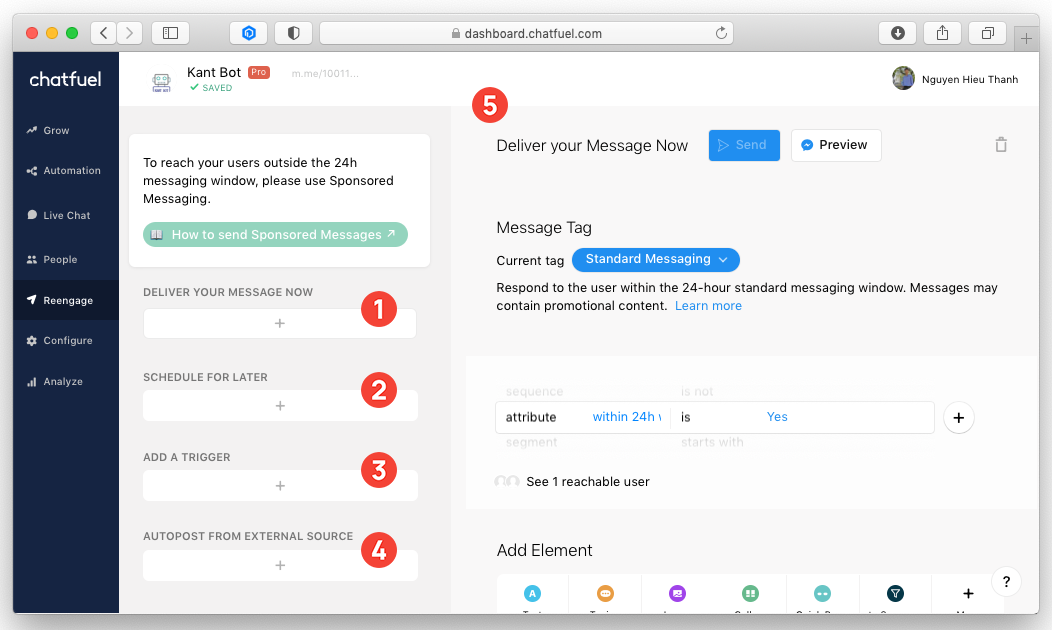
\includegraphics[width=15cm]{chatfuel/re-engage}
	\caption{Giao diện danh sách người dùng đã tương tác với bot}
	\label{fig:fig-c3-re-engage}
\end{figure}\par

\subsection{Thiết kế một cuộc hội thoại với Chatfuel}
\subsubsection{Thiết kế chatbot bằng blocks}
Một block được sử dụng là một giai đoạn của cuộc hội thoại. Lần đầu truy cập, chatbot sẽ có 02 block mặc định là \textit{tin nhắn chào mừng} (welcome message) và \textit{câu trả lời mặc định} (default answer) (xem hình \ref{fig:fig-c3-blocks}). Đúng như tên gọi, \textit{tin nhắn chào mừng} được gửi lần đầu tiên khi người dùng bắt đầu trò chuyện với bot và \textit{câu trả lời mặc định} dùng để gửi đi khi bot không hiểu tin nhắn của người dùng.\par
Ở giao diện làm việc với blocks, để tạo một block mới, ta chọn dấu cộng (+) ở khung \textbf{(1)}, hoặc tạo một nhóm các block bằng việc chọn \textit{+ ADD SEQUENCE OR GROUP} sau đó đặt tên cho nhóm. Ngoài ra, các block có thể được phân nhóm và sắp xếp dễ dàng bằng thao tác kéo thả chuột.\par
Chọn một block ở khung danh sách \textbf{(1)} để hiện nội dung của block (hình \ref{fig:fig-c3-block-demo}). Tại đây, tên block được hiển thị ở \textbf{(1)}, người dùng có thể nhấn chuột vào để đổi tên block theo ý mình. Tiếp sau tên block là nút \textit{LINK} dùng để tạo \textit{đường dẫn} (URL) để truy cập trực tiếp tới block đó. Phần \textbf{(2)} là thông tin các đường vào/ra của block, trên hình \ref{fig:fig-c3-block-demo}, người dùng có thể truy cập tới block từ menu chính của fanpage, từ \textit{câu trả lời mặc định} và từ một block/flow có tên \textit{f\_survey}; cũng vậy, từ block \textit{menu} có thể chuyển sang các block/flow có tên \textit{about-bot}, \textit{start}, \textit{update-information} và \textit{open-form}. Tiếp theo là nội dung chính hay kịch bản của block \textbf{(3)} và cuối cùng là các thành \textit{thành phần} (elements) để thiết kế block, còn được gọi là các phug-in \textbf{(4)}.\par
\begin{figure}[htb!]\centering
	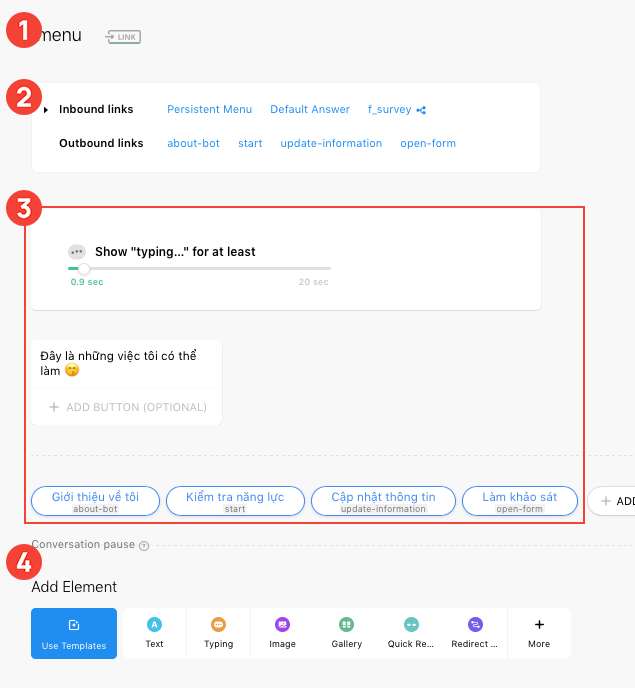
\includegraphics[width=10cm]{chatfuel/block-demo}
	\caption{Nội dung của một block}
	\label{fig:fig-c3-block-demo}
\end{figure}\par

Khi chọn \textit{More} để hiển thị danh sách đầy đủ (hình \ref{fig:fig-c3-block-elements-list}), các plug-in này sẽ được hiển thị theo các nhóm chức năng chính, cụ thể:
\begin{itemize}
	\item \textbf{Add \& Send Content:} nhóm phug-in này đơn giản và dễ sử dụng nhất, giúp quản trị viên thêm và gửi nội dung từ block: \begin{itemize}
		\item \textbf{Text}: Cho phép tạo ra một tin nhắn văn bản, tối đa 640 ký tự. Plug-in này hỗ trợ mã hóa văn bản UTF-8 do đó có thể được sử dụng cho nhiều ngôn ngữ khác nhau, trong đó có tiếng Việt.
		\item \textbf{Typing}: Plugin này tạo ra một hoạt ảnh đang nhập tin nhắn cho người dùng trong khoảng thời gian đặt trước: từ $0.1$ đến $20$ giây. Hoạt ảnh này cho người dùng thời gian để đọc tin nhắn từ bot trước khi tin nhắn tiếp theo được gửi. Để bot mô phỏng hành động giống với người thật, Chatfuel khuyến nghị chọn số giây khớp với số dòng của tin nhắn trước đó. Ví dụ, tin nhắn trước đó có 04 dòng, thì hoạt ảnh này nên được đặt là 4 giây.
		\item \textbf{Image}: Cho phép thêm hình ảnh (cả ảnh tĩnh và ảnh động) vào block với các định dạng được chấp nhận là PNG, JPG và GIF. Để thời gian gửi ảnh được tối ưu, hình ảnh được lựa chọn nên có kích thướt và dung lượng vừa phải, cụ thể: $500\times 500$ pixel cho hình ảnh tỉ lệ $1:1$ hoặc $854\times 460$ pixel cho hình ảnh tỉ lệ $16:9$ và kích thước tệp không lớn hơn 1 MB; đối với ảnh động (GIF), tốc độ khung hình (frames per second) tối đa là 60 FPS và kích thước tệp không lớn hơn 2 MB.
		\item \textbf{Gallery}: Plug-in này cung cấp một thư viện cho bot (hình \ref{fig:fig-s3-8-chatfuel-gallery}). \textit{Thư viện} là một màn hình hiển thị theo chiều ngang chứa nhiều hình ảnh mà người dùng có thể cuộn qua (tối đa 10 hình ảnh), mỗi hình ảnh đều có \textit{tiêu đề} (title), \textit{tiêu đề phụ} (subtitle), URL và (các) nút nhấn. Plug-in này có thể sử dụng cho việc giới thiệu sản phẩm, hiển thị các tùy chọn, hiển thị các \textit{câu hỏi thường gặp}... Các nút nhấn cho mỗi mục trong thư viện có thể chuyển hướng người dùng đến một block/flow khác, mở URL, thực hiện cuộc gọi đến một số cụ thể...\par
		\begin{figure}[htb!]\centering
			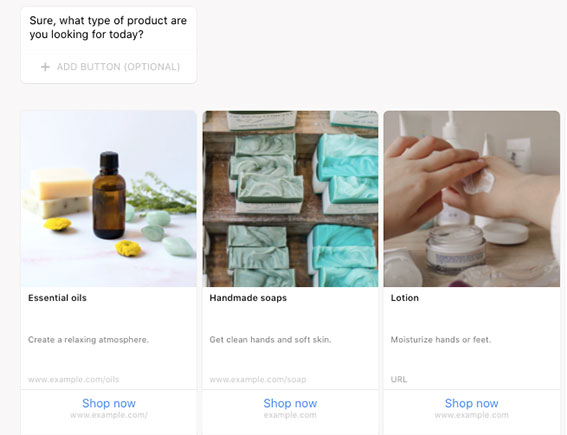
\includegraphics[width=12cm]{chatfuel/gallery}
			\caption{Một thư viện được tạo ra từ Chatfuel}
			\label{fig:fig-s3-8-chatfuel-gallery}
		\end{figure}
		\item \textbf{Video}: Cho phép thêm video vào một khối. Tuy nhiên, trước tiên cần tải video lên Facebook hoặc Dropbox và bật chia sẻ công khai trên nền tảng tương ứng đó, nghĩa là video được hiển thị cho bất kỳ ai có liên kết. Với video, định dạng tệp phải là MP4 với kích thước tệp tối đa là 25 MB.
		\item \textbf{Audio}: Cho phép thêm một tệp âm thanh vào block. Cũng như video, tệp âm thanh cần được tải lên một dịch vụ lưu trữ nào đó và đặt ở chế độ công khai. Các định dạng được hỗ trợ là MP3, WAV và OGG với kích thước tệp tối đa là 25 MB.
		\item \textbf{Comment}: Dùng để thêm một ghi chú vào các phần tử của chatbot. Comment sẽ không hiển thị cho người dùng. Thêm chúng để tạo ghi chú để chỉnh sửa về sau hoặc để lại ghi chú cho những người quản trị khác.
	\end{itemize}
	\item \textbf{Collect User Data}: Thu thập dữ liệu từ người dùng để phân loại hoặc tiếp cận trong tương lai. \begin{itemize}
		\item \textbf{Quick Reply}: Plug-in này cho phép thêm các tùy chọn phản hồi vào bên dưới của plug-in \textit{Text} (hình \ref{fig:fig-s3-9-chatfuel-quick-reply}). Mỗi tùy chọn trả lời nhanh có thể bao gồm tối đa 20 ký tự văn bản và biểu tượng cảm xúc, và có thể có tối đa 11 câu trả lời nhanh. Khi được nhấn vào, các câu trả lời này có thể kích hoạt phản hồi của AI, dẫn người dùng đến một khối khác và thậm chí lưu phản hồi của họ vào một thuộc tính.\par
		\begin{figure}[htb!]\centering
			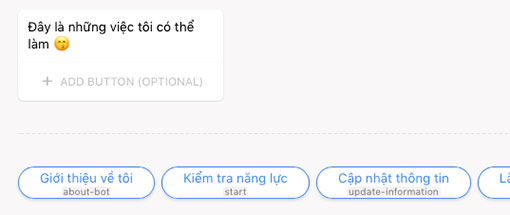
\includegraphics[width=10cm]{chatfuel/quick-reply}
			\caption{Minh họa các câu trả lời nhanh}
			\label{fig:fig-s3-9-chatfuel-quick-reply}
		\end{figure}
		\item \textbf{Save User Input}: Cho phép lấy văn bản hoặc tệp từ người dùng của chatbot. Bot có thể tự động lưu tin nhắn vắn bản vào một thuộc tính hoặc tự động gửi tới email của quản trị viên bằng plug-in \textbf{Notify Admin Via Email} hoặc tới bảng tính bằng plug-in \textbf{Save to Google Sheets}. Plug-in này có thể chấp nhận bất kỳ loại tệp nào (DOCX, XLSX, PDF, JPG, v.v.) được phép gửi ở Facebook hay Facebook Messenger.
		\item \textbf{Set User Attribute}: Plug-in này sẽ tự động đặt giá trị thuộc tính (tùy chỉnh) cho người dùng dựa trên việc họ đã xem một phần nhất định của chatbot hay chưa, hoặc thêm các trường dữ liệu vào thông tin người dùng. Chatfuel hỗ trợ đặt bất kỳ giá trị nào, nhưng tập hợp điển hình có thể bao gồm \textit{có} (yes), \textit{không} (no) hoặc \textit{không được đặt} (unset). Từ đó, ta có thể thiết lập một chuỗi để chỉ gửi cho những người dùng đã nhìn thấy một khối nhất định.
		\begin{minipage}{\linewidth}
		\begin{wrapfigure}{r}{5cm}\centering
			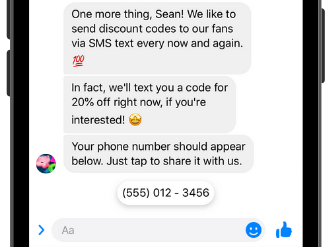
\includegraphics[width=5cm]{chatfuel/save-phone-number.png}
			\caption{Minh họa plug-in \textit{Save User Phone~Number/Email}}
			\label{fig:fig-s3-10-chatbot-ask-for-phone-number}
		\end{wrapfigure}
		\item \textbf{Save User Phone Number} và \textbf{Save User Email}: Cho phép lưu lại số điện thoại/email của người dùng và lưu nó vào một thuộc tính để sử dụng sau này. Plug-in tạo ra kèm với một tin nhắn mặc định yêu cầu thông tin, quản trị viên có thể giữ nguyên hoặc tùy chỉnh.\begin{itemize}
			\item[+] Nếu thông tin của người dùng được hiển thị công khai trên hồ sơ Facebook, họ sẽ thấy thông tin đó tự động điền dưới dạng \textit{câu trả lời nhanh} khi bot yêu cầu. Họ có thể chọn hoặc nhập thông tin khác.
			\item[+] Nếu số điện thoại của người dùng không hiển thị công khai trên hồ sơ Facebook, họ có thể nhập thông tin đó theo cách thủ công khi bot yêu cầu.
		\end{itemize}
		\end{minipage}
	\end{itemize}
	\item \textbf{Export \& Import}: Các plug-in trong phần này cho phép bot xử lý dữ liệu bằng cách gửi đi hoặc gọi về từ một nguồn bên ngoài. \begin{itemize}
		\item \textbf{JSON API}: Cho phép thực hiện các yêu cầu đến máy chủ của bên thứ ba để nhận về dữ liệu dạng JSON. Từ đó bot có thể hiển thị tệp hình ảnh, âm thanh hoặc video cho người dùng hoặc gửi thuộc tính đến máy chủ để lưu trữ.
		\item \textbf{Save to Google Sheets}: Cho phép xuất dữ liệu của người dùng sang bảng tính (Google Sheets). Chọn một hoặc nhiều thuộc tính hiện có trong bot và các giá trị người dùng cho từng thuộc tính (thậm chí các giá trị được thu thập từ các plug-in như \textbf{Save User Input}) sẽ được gửi đến bảng tính ngay lập tức khi chúng được thu thập.
		\item \textbf{Notify Admin via Email}: Plug-in này sẽ gửi một email theo mẫu đến (các) địa chỉ email được chỉ định và sẽ điền vào bất kỳ thuộc tính nào được liệt kê với các giá trị cho một người dùng cụ thể. Plug-in này chỉ để gửi thông tin người dùng đến quản trị viên bot, không dùng để gửi email cho người dùng. Ví dụ khi bot nhận được một đơn xin việc (application), với email mẫu như hình \ref{fig:fig-s3-11-chatfuel-notify-admin-via-email}, quản trị viên sẽ nhận được email với dữ liệu được điền, như \textit{"You've got a new applicant for Marketing Associate position. Their name is Lawrence Smith and their phone number is 555-123-4567."}\par
		\begin{figure}[htb!]\centering
			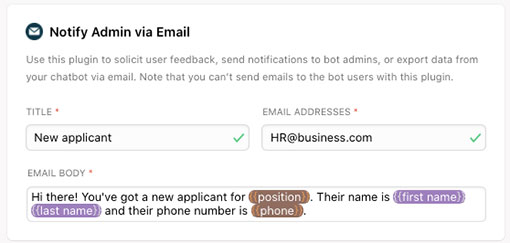
\includegraphics[width=11cm]{chatfuel/notify-admin-via-email}
			\caption{Thiết lập gửi email cho quản trị viên}
			\label{fig:fig-s3-11-chatfuel-notify-admin-via-email}
		\end{figure}\par
		\item \textbf{Export/Import Content via Zapier}: Cho phép nhập, xuất dữ liệu từ một bên thứ ba (Google Sheets, MailChimp, Shopify, Zoom...).
	\end{itemize}
	\item \textbf{Redirect Users}: Chuyển hướng người dùng sang block/flow khác dựa trên hành động của họ hoặc các thuộc tính đã gán. \begin{itemize}
		\item \textbf{Redirect to Block}: Cho phép chuyển hướng người dùng của chatbot đến bất kỳ block/flow nào. Hơn nữa, phug-in này có thể thực hiện chuyển hướng nâng cao dựa trên các thuộc tính người dùng – nghĩa là có thể gửi những người dùng đáp ứng các tiêu chí nhất định đến các khối nhất định.
		\item \textbf{Subscribe/Unsubscribe to Sequence}: Cho phép người dùng đăng ký/hủy đăng ký nhận thông báo thuộc một nhóm nào đó. Việc này diễn ra hoàn toàn tự động khi người dùng truy cập đến khối có chứa plug-in này.
		\item \textbf{A/B Testing}: Plugin này cho phép thử nghiệm các phiên bản khác nhau của block trong chatbot. Nó sẽ đưa một số người dùng đến một phiên bản và những người dùng còn lại đến một phiên bản khác, từ đó có thể xem phiên bản nào hoạt động tốt nhất. Quản trị viên có thể chọn tỷ lệ phần trăm người dùng muốn gửi cho mỗi phiên bản.
	\end{itemize}
	\item \textbf{Connect Users to a Human}: Kết nối người dùng với quản trị viên để trao đổi trực tiếp. \begin{itemize}
		\item \textbf{Live Chat}: Cho phép kết nối người dùng với một phiên chat trực tiếp với quản trị viên. Các chức năng tự động của chatbot sẽ dừng lại cho tới khi phiên chat kết thúc. Ngoài ra, plug-in cho phép thiết lập thời gian người dùng chờ để quay lại với bot tự dộng.
		\item \textbf{Conversation Handover}: Plug-in này cho phép định cấu hình các ứng dụng khác để xử lý các phiên trò chuyện trực tiếp do người dùng bot yêu cầu. Sử dụng nó khi cần trả lời người dùng từ Hộp thư đến của Facebook hoặc từ ứng dụng của bên thứ ba như hệ thống CRM (customer relationship management). Sau khi một cuộc trò chuyện được chuyển giao cho ứng dụng, các chức năng tự động của bot sẽ tạm dừng cho đến khi người dùng quay lại với nó.
	\end{itemize}
\end{itemize}
\begin{figure}[htb!]\centering
	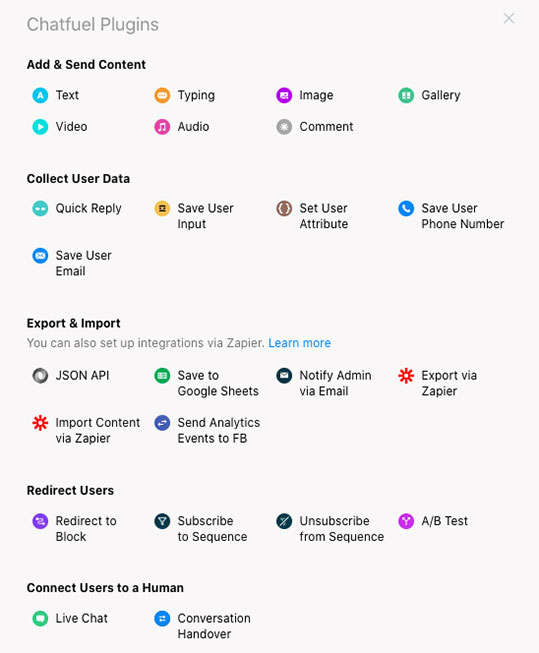
\includegraphics[width=10cm]{chatfuel/block-elements-list}
	\caption{Danh sách các plug-in của block}
	\label{fig:fig-c3-block-elements-list}
\end{figure}

\subsubsection{Thiết kế chatbot bằng flows}
Không như block, \textit{flows} có thể đảm nhận một mảng chức năng, hoặc thậm chí toàn bộ chức năng của một chatbot do được trang bị cơ chế điều hướng và các cấu trúc rẽ nhánh rất linh hoạt. Hơn nữa, flow được thiết kế thông qua việc kéo thả các thẻ trực quan, thay vì giao diện tuyến tính của block. Khi làm việc với flow, có thể dễ dàng nhận ra flow bao gồm nhiều thẻ, mỗi thẻ tương tự với một block và được liên kết liên tục với nhau tạo thành một tiến trình hội thoại.\par
Có 06 loại thẻ có thể tạo ra trong một flow: \begin{itemize}
	\item \textbf{Send message}: Thẻ này thực hiện gửi tin nhắn đến người dùng, bao gồm: tin nhắn văn bản, hình ảnh, hoạt ảnh đang nhập tin nhắn, thư viện, video, âm thanh, trả lời nhanh, lưu điện thoại/email của người dùng.
	\item \textbf{Action}: Thẻ thực hiện các hành động, như: đặt/xóa thuộc tính người dùng, thông báo tới quản trị viên, gọi JSON API. Sử dụng thẻ này khi muốn thực hiện một hành động ngầm, như lưu, thay đổi hoặc gửi dữ liệu.
	\item \textbf{Split traffic}: Thực hiện chức năng tương tự plug-in \textbf{A/B Testing} của block.
	\item \textbf{Condition}: Tạo ra một cấu trúc rẽ nhánh để chuyển hướng người dùng dựa trên (các) điều kiện của thuộc tính.
	\item \textbf{Delay}: Trì hoãn cuộc hội thoại trong một khoảng thời gian xác định.
	\item \textbf{Redirect to Flow/Block}: Chuyển hướng người dùng sang một block/flow khác.
\end{itemize}
Ngoài thẻ, flow còn có các liên kết để điều hướng cuộc hội thoại và liên kết các thẻ. Các vòng tròn nhỏ ở góc dưới cùng bên phải của thẻ và ở phía bên phải của các nút nhấn là những điểm mà từ đó có thể vẽ ra các mũi tên để kết nối các khối. Các mũi tên liên kết các phần khác nhau của cuộc trò chuyện với nhau, hiển thị cho bot biết nơi đưa người dùng tiếp theo.\par
Có hai cách để thiết kế một flow: \begin{enumerate}[label=\textbf{\arabic*.}]
	\item Thiết kế bố cục cơ bản bằng các thẻ trước, sau đó thực hiện tạo các liên kết.
	\item Thiết kế bố cục khi thực hiện bằng cách thêm từng thẻ một. Xây dựng khối đầu tiên, sau đó nhấp vào hình tròn liên kết, một menu xuất hiện để chọn loại thẻ tiếp theo cần thiết kế.
\end{enumerate}\par
Tuy nhiên, tuy hỗ trợ cấu trúc rẽ nhánh mạnh mẽ và các plug-in của block được kế thừa hoàn toàn, flows vẫn có một nhược điểm lớn là trình thiết kế của nó dựa trên nền WebGL, mà hiệu suất làm việc là một điều đáng lưu tâm, đặc biệt với những flow phức tạp. Do đó, nên cân nhắc và sử dụng linh hoạt qua lại giữa block và flow.\par

\subsection{Thiết kế chatbot thông qua JSON API}
Như đã nói ở phần trước, plug-in JSON API cho phép tích hợp chương trình, thuật toán phức tạp thông qua việc gửi và nhận các yêu cầu (bao gồm cả phương thức GET và POST) từ máy chủ cá nhân được lập trình sẵn. Cụ thể, JSON API có thể:\begin{itemize}
	\item Tạo ra nội dung động (do phần code phát sinh).
	\item Lấy và đặt các thuộc tính người dùng.
	\item Chuyển hướng người dùng sang block/flow khác.
\end{itemize}\par
Phản hồi của máy chủ có thể kết hợp nhiều dạng tin nhắn với nhau trong một biến JSON, hoặc không phản hồi bất cứ nội dung gì để dừng JSON. Sau khi chọn plug-in JSON API, một bảng chọn tương tự hình \ref{fig:fig-c3-json-api} được thêm vào block/flow. Cần thiết lập các dữ liệu sau đây: \begin{enumerate}[label=\textbf{(\arabic*)},align=left,left=0cm..0cm,itemindent=*]
	\item \textbf{Method}: Phương thức của \textit{yêu cầu} (request) được gửi đi: GET hoặc POST.
	\item \textbf{URL}: địa chỉ của máy chủ nhận request. Nếu chọn phương thức GET thì thêm dữ liệu vào sau URL.
	\item Nhấn chọn \textit{Test the Request} để kiểm tra kết quả.
	\item \textbf{Response}: kết quả phản hồi từ máy chủ.
\end{enumerate}\par

\begin{figure}[htb!]\centering
	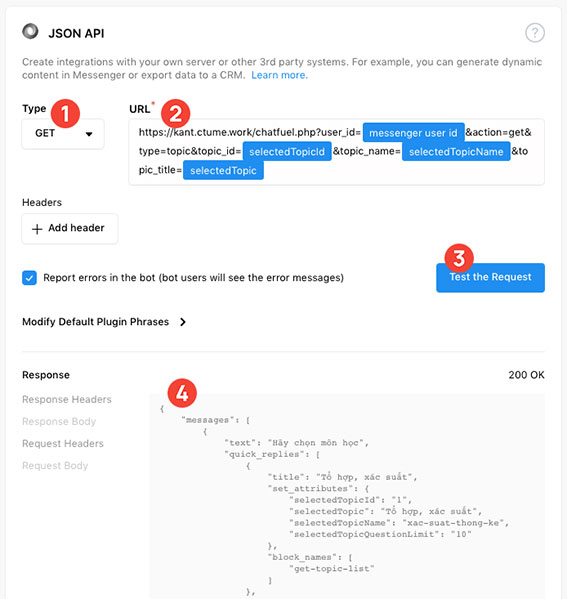
\includegraphics[width=14cm]{chatfuel/json-api}
	\caption{JSON API}
	\label{fig:fig-c3-json-api}
\end{figure}\par

Dưới đây là cú pháp JSON hợp lệ dùng để ra lệnh cho chatbot.
\subsubsection{Gửi văn bản}
Sử dụng cú pháp sau để gửi tin nhắn văn bản.
\begin{lstlisting}
{
	"messages": [
		{ "text": "Welcome to the Chatfuel Rockets!" },
		{ "text": "What are you up to?" }
	]
}
\end{lstlisting}\par

\subsubsection{Gửi hình ảnh}
Sử dụng cú pháp dưới đây để gửi hình ảnh. Facebook Messenger hỗ trợ định dạng JPG, PNG và GIF.
\begin{lstlisting}
{
	"messages": [
		{
			"attachment": {
				"type": "image",
				"payload": {
					"url": "https://rockets.chatfuel.com/assets/welcome.png"
				}
			}
		}
	]
}
\end{lstlisting}\par
Ngoài ra, Chatfuel còn hỗ trợ chia sẻ hình ảnh từ một bài viết Facebook thay vì tải lên thủ công:
\begin{lstlisting}
{
	"messages": [
		{
			"attachment": {
				"type": "template",
				"payload": {
					"template_type": "media",
					"elements": [
						{
							"media_type": "image",
							"url": "https://www.facebook.com/chatfuelrockets/photos/1087668107975064",
							"buttons": [
								{
									"title": "Go to Chatfuel!",
									"type": "web_url",
									"url": "https://chatfuel.com/"
								}
							]
						}
					]
				}
			},
			"quick_replies": [
				{
					"title": "That's cool!",
					"set_attributes": {
						"feedback": "Cool!"
					}
				}
			]
		}
	]
}
\end{lstlisting}\par

\subsubsection{Gửi video}
Cú pháp JSON dưới đây dùng để gửi một video. Facebook Messenger hỗ trợ video định dạng MP4, với kích thướt tối đa là 25 MB.
\begin{lstlisting}
{
	"messages": [
		{
			"attachment": {
				"type": "video",
				"payload": {
					"url": "https://rockets.chatfuel.com/assets/video.mp4"
				}
			}
		}
	]
}
\end{lstlisting}\par

Cũng như với hình ảnh, JSON sau đây có thể chia sẻ một video từ bài đăng Facebook thay vì tải lên thủ công:
\begin{lstlisting}
{
	"messages": [
		{
			"attachment": {
				"type": "template",
				"payload": {
					"template_type": "media",
					"elements": [
						{
							"media_type": "video",
							"url": "https://www.facebook.com/chatfuelrockets/videos/252894858962779/",
							"buttons": [
								{
								"title": "Go to Chatfuel!",
								"type": "web_url",
								"url": "https://chatfuel.com/"
								}
							]
						}
					]
				}
			},
			"quick_replies": [
				{
					"title": "That's cool!",
					"set_attributes": {
						"feedback": "Cool!"
					}
				}
			]
		}
	]
}
\end{lstlisting}\par

\subsubsection{Gửi âm thanh}
Sử dụng cú pháp này để gửi các tệp âm thanh. Facebook Messenger hỗ trợ âm thanh MP3, OGG, WAV, có dung lượng tối đa 25 MB.
\begin{lstlisting}
{
	"messages": [
		{
			"attachment": {
				"type": "audio",
				"payload": {
					"url": "https://rockets.chatfuel.com/assets/hello.mp3"
				}
			}
		}
	]
}
\end{lstlisting}\par

\subsubsection{Gửi tệp}
Sử dụng cú pháp này để gửi bất kỳ tệp nào khác, với kích thướt tối đa 25 MB.
\begin{lstlisting}
{
	"messages": [
		{
			"attachment": {
				"type": "file",
				"payload": {
					"url": "https://rockets.chatfuel.com/assets/ticket.pdf"
				}
			}
		}
	]
}
\end{lstlisting}\par

\subsubsection{Gửi thư viện}
Sử dụng cú pháp này để gửi một thư viện (có thể cuộn ngang). Mỗi mục bao gồm một hình ảnh, mô tả ngắn và các nút nhấn.
\begin{lstlisting}
{
	"messages": [
		{
			"attachment": {
				"type": "template",
				"payload": {
					"template_type": "generic",
					"image_aspect_ratio": "square",
					"elements": [
						{
							"title": "Chatfuel Rockets Jersey",
							"image_url": "https://rockets.chatfuel.com/assets/shirt.jpg",
							"subtitle": "Size: M",
							"buttons": [
								{
									"type": "web_url",
									"url": "https://rockets.chatfuel.com/store",
									"title": "View Item"
								}
							]
						},
						{
							"title": "Chatfuel Rockets Jersey",
							"image_url": "https://rockets.chatfuel.com/assets/shirt.jpg",
							"subtitle": "Size: L",
							"default_action": {
								"type": "web_url",
								"url": "https://rockets.chatfuel.com/store"
							},
							"buttons": [
								{
									"type": "web_url",
									"url": "https://rockets.chatfuel.com/store",
									"title": "View Item"
								}
							]
						}
					]
				}
			}
		}
	]
}
\end{lstlisting}\par

Thuộc tính \texttt{image\_aspect\_ratio} có thể mang giá trị \texttt{square} (vuông) hoặc \texttt{horizontal} (ngang), giá trị \texttt{horizontal} là mặc định.\par

\subsubsection{Gửi hóa đơn}
Sử dụng cú pháp này để gửi một tin nhắn xác nhận đơn đặt hàng. Bao gồm phần tóm tắt đơn đặt hàng, chi tiết thanh toán và thông tin vận chuyển.
\begin{lstlisting}
{
	"messages": [
		{
			"attachment": {
				"type": "template",
				"payload": {
					"template_type": "receipt",
					"recipient_name": "Mark Zuckerberg",
					"order_number": "12345678901",
					"currency": "USD",
					"payment_method": "Visa 2345",
					"order_url": "https://rockets.chatfuel.com/store?order_id=12345678901",
					"timestamp": "1428444666",
					"address": {
						"street_1": "1 Hacker Way",
						"street_2": "",
						"city": "Menlo Park",
						"postal_code": "94025",
						"state": "CA",
						"country": "US"
					},
					"summary": {
						"subtotal": 105,
						"shipping_cost": 4.95,
						"total_tax": 9,
						"total_cost": 118.95
					},
					"adjustments": [
						{
							"name": "CF Rockets Superstar",
							"amount": -25
						}
					],
					"elements": [
						{
							"title": "Chatfuel Rockets Jersey",
							"subtitle": "Size: M",
							"quantity": 1,
							"price": 65,
							"currency": "USD",
							"image_url": "http://rockets.chatfuel.com/assets/shirt.jpg"
						},
						{
							"title": "Chatfuel Rockets Jersey",
							"subtitle": "Size: L",
							"quantity": 1,
							"price": 65,
							"currency": "USD",
							"image_url": "http://rockets.chatfuel.com/assets/shirt.jpg"
						}
					]
				}
			}
		}
	]
}
\end{lstlisting}
